
\title{T-61.5130 Machine Learning and Neural Networks}
\author{Karhunen, Luttinen}
\date{Exercise 11, 13.12.2012}

\newcommand{\vect}[1]{{\bf{#1}}}
\newcommand{\svect}[1]{\boldsymbol{#1}}
\newcommand{\matr}[1]{\boldsymbol{#1}}


\begin{document}

\maketitle

\begin{enumerate}

\item In this problem we consider the optimized form of the learning
  vector quantization algorithm developed by Kohonen.
  \begin{enumerate}
  \item The Voronoi vector closest to the input vector $\mathbf{x}(n)$
    is updated as
    \begin{equation}
      \mathbf{w}_c(n+1)=\mathbf{w}_c(n)+\alpha_c(n)[\mathbf{x}(n)-\mathbf{w}_c(n)]
      \label{equation: 1}
    \end{equation}
    if the classification is correct, or as
    \begin{equation}
      \mathbf{w}_c(n+1)=\mathbf{w}_c(n)-\alpha_c(n)[\mathbf{x}(n)-\mathbf{w}_c(n)]
      \label{equation: 2}
    \end{equation}
    if the classification is incorrect.  The other Voronoi vectors
    remain unchanged.  Show that these rules may be integrated into a
    single equation, as follows:
    \begin{equation}
      \mathbf{w}_j(n+1) = (1-s_j(n)\alpha_j(n)) \mathbf{w}_j(n) + s_j(n)
      \alpha_j(n) \mathbf{x}(n).
      \label{equation: 3}
    \end{equation}
    In the above equations, $0<\alpha_j(n)<1$ is a learning constant
    for $\mathbf{w}_j$, and $s_j(n)$ is a sign function depending on
    the classification result of the $n$-th input vector
    $\mathbf{x}(n)$: For the closest Voronoi vector, $s_j(n)=+1$ if
    classification is correct and $s(n)=-1$ if classification is
    incorrect.  For the other Voronoi vectors, $s_j(n)=0$.

  \item We wish to arrange for the effects of the corrections to the
    Voronoi vectors, made at different times, to have equal influence
    when referring to the end of the learning period.  Show that this
    optimization criterion described at the beginning of the problem
    is satisfied if
    \begin{equation*}
      \alpha_j(n)=(1-s_j(n)\alpha_j(n))\alpha_j(n-1)
    \end{equation*}
    which yields the optimized value of the learning constant
    $\alpha_j(n)$ as
    \begin{equation*}
      \alpha_j^{\text{opt}}(n) = \frac {\alpha_j^{\text{opt}}(n-1)} {1
        + s_j(n) \alpha_j^{\text{opt}}(n-1)}.
    \end{equation*}
    Note that $\alpha_j(n)=\alpha_j(n-1)$ if the $j$-th Voronoi vector
    was not closest to the input vector $\mathbf{x}(n)$.
  \end{enumerate}

  \begin{solution}

    \begin{enumerate}
    \item 

      First, re-organize the terms in \eqref{equation: 3}:
      \begin{align*}
        \mathbf{w}_j(n+1) &= (1-s_j(n)\alpha_j(n)) \mathbf{w}_j(n) +
        s_j(n)\alpha_j(n)\mathbf{x}(n)
        \\
        &= \mathbf{w}_j(n) + s_j(n) \alpha_j(n) [\mathbf{x}(n) -
        \mathbf{w}_j(n)].
      \end{align*}
      The update equations \eqref{equation: 1} and \eqref{equation: 2}
      are obtained by inserting $s_j(n)=1$ and $s_j(n)=-1$,
      respectively.  The Voronoi vector remains unchanged by inserting
      $s_j(n)=0$.
      % This is seen by inserting $s_n=1$ and $s_n=-1$ into
      % equation (\ref{equation: 3}) yielding the two update equations
      % (\ref{equation: 1}) and (\ref{equation: 2}).

    \item 

      For the LVQ equation we note that the updated weight vector
      $\mathbf{w}_j(n+1)$ contains a ``trace'' from $\mathbf{x}(n)$ by
      virtue of the last term $s_j(n)\alpha_j(n)\mathbf{x}(n)$.
      Moreover, it contains traces of previous samples, namely,
      $\mathbf{x}(n-1)$, $\mathbf{x}(n-2),\;\ldots,\; \mathbf{x}(1)$
      by virtue of the present value of the weight vector
      $\mathbf{w}_j(n)$.

      Consider $\mathbf{w}_j(n)$ which is defined by
      \begin{equation}
        \mathbf{w}_j(n) = [1 - s_j(n-1) \alpha_j(n-1)]
        \mathbf{w}_j(n-1) + s_j(n-1) \alpha_j(n-1) \mathbf{x}(n-1).
        \label{eq:lvq2}
      \end{equation}
      Hence, substituting equation \eqref{eq:lvq2} into the LVQ
      equation \eqref{equation: 3} and combining terms yields
      \begin{align*}
        \mathbf{w}_c(n+1) &= \left[1 - s_j(n) \alpha_j(n)\right]
        \left[1 - s_j(n-1) \alpha_j(n-1)\right] \mathbf{w}_j(n-1) +
        \\
        &\qquad \left[1 - s_j(n) \alpha_j(n)\right] s_j(n-1)
        \alpha_j(n-1) \mathbf{x}(n-1) + s_j(n) \alpha_j(n)
        \mathbf{x}(n).
        %\label{eq:lvq3}
      \end{align*}
      It follows therefore that the effect of $\mathbf{x}(n-1)$ on the
      updated weight vector $\mathbf{w}_j(n+1)$ is scaled by the
      factor $(1-s_j(n)\alpha_j(n)) s_j(n-1) \alpha_j(n-1)$. On the
      other hand, the effect of $\mathbf{x}(n)$ is scaled by
      $s_j(n)\alpha_j(n)$.  Accordingly, if we require that
      $\mathbf{x}(n)$ and $\mathbf{x}(n-1)$ are to have the same
      effect on $\mathbf{w}_j(n+1)$, then we must have
      \begin{equation*}
        | s_j(n) \alpha_j(n) |= | (1-s_j(n)\alpha_j(n))\alpha_j(n-1) s_j(n-1) |.
      \end{equation*}
      If $s_j(n-1)$ and $s_j(n)$ are either $1$ or $-1$, their
      absolute values are $1$. The remaining quantities inside the
      absolute values are positive and we obtain
      \begin{equation*}
        \alpha_j(n) = (1-s_j(n)\alpha_j(n))\alpha_j(n-1) .
      \end{equation*}
      Solving for $\alpha_j(n)$, we get the optimum
      \begin{equation}
        \alpha_j^{opt}(n) = \frac {\alpha_j^{opt}(n-1)} {1 +
          s_j(n)\alpha_j^{opt}(n-1)}. \label{eq:alpha_opt}
      \end{equation}
      (If $s_j(n)=0$, $\alpha_j(n)$ remains unchanged by
      \eqref{eq:alpha_opt}.  If $s_j(n-1)=0$, $\mathbf{x}(n-1)$ is
      properly ignored by \eqref{eq:alpha_opt}.)


    \end{enumerate}

  \end{solution}
  

\item Using the LMS algorithm, formulate a learning algorithm for the
  focused neuronal filter, which is drawn in the figure:
    \begin{center}
      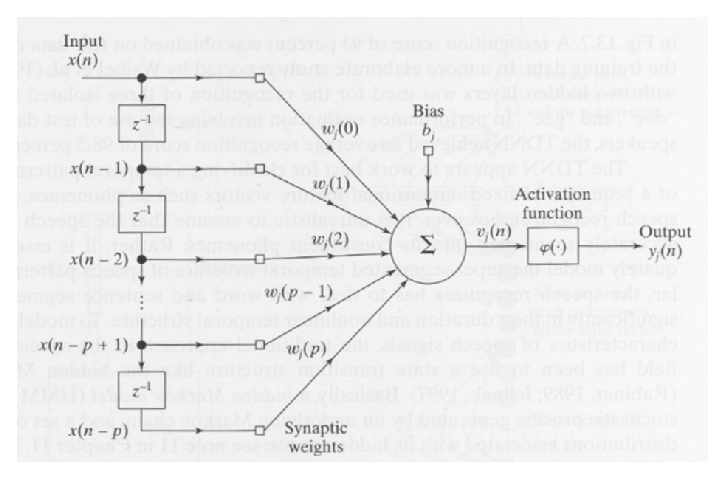
\includegraphics[width=11cm]{l12k3a}
    \end{center}


  \begin{solution}

    The output of the filter is $y(n) =
    \varphi(v(n))$, where $v(n)$ is the linear response of the neuron $$v(n) = b +
    \sum_{l=0}^p w(l) x(n-l) \, .$$ (Notice that for convenience we use
    a simpler notation, where the index of the neuron is dropped.)
    The least mean square (LMS) algorithm aims at minimising the mean
    square error $$\mathcal{E} = \sum_n \mathcal{E}(n) = \frac{1}{2} \sum_n e(n)^2 \, ,$$
    where $e(n) = d(n) - y(n)$ is the error made by the network.  For deriving an
    on-line learning algorithm we  use the stochastic
    gradient descent method where one proceeds in the direction of the negative
    gradient of the instantaneous
    error $\mathcal{E}(n)$.

    From the chain rule we have $$\frac{\partial \mathcal{E}(n)}{\partial w(l)} =
    \frac{\partial \mathcal{E}(n)}{\partial e(n)} \frac{\partial e(n)}{\partial
      y(n)} \frac{\partial y(n)}{\partial v(n)} \frac{\partial
      v(n)}{\partial w(l)} = e(n) (-1) \varphi'(v(n)) x(n-l) \, .$$ 
    $\varphi'$ denotes the derivative of the activation function.
    The
    learning rule for adjusting the weight $w_l$ is thus $\Delta w_l = -\eta \partial \mathcal{E}(n) / \partial
    w(l) = \eta e(n) \varphi'(v(n)) x(n-l)$, where $\eta$ is the learning
    rate.  A similar derivation for the bias $b$ will give the learning
    rule $\Delta b = - \eta \partial \mathcal{E}(n) / \partial b = \eta e(n)
    \varphi'(v(n))$.
    % }

  \end{solution}
  
\item How would you design a tapped delay line for a focused time
  lagged feedforward network?


  \begin{solution}

    Once the structure is fixed, the parameters can be learned for
    instance by temporal back-propagation.  For the design of the structure there are no
    general rules.  Cross-validation, Bayesian models selection etc.
    can be used but the structure of the delay line has very many
    degrees of freedom.

    The available prior knowledge about the plausible time lags should
    be used for choosing the lengths of the delays, possible averaging
    lengths and so on.  Often it is reasonable to have a higher
    resolution for the immediate past and increasingly coarse
    resolution for more distant past.


  \end{solution}
  
\item Discuss how the temporal back-propagation algorithm may be used for the
  training of a distributed time lagged feedforward network (TLFN) for single-step prediction.

  \begin{solution}

    Let $\mathbf{x}(n)=[x(n), x(n-1), \ldots ,x(n-p)]$ denote the
    vector of current and delayed input signals applied to the
    distributed TLFN at time $n$. Let $y(n)$ denote the actual
    response of the network trained using the temporal
    back-propagation algorithm. With one-step prediction as the
    requirement, the desired response is the value of the input signal
    one step into the future, that is,
    \begin{equation*}
      y(n) = x(n+1).
    \end{equation*}
    With these provisions, we may then proceed with the temporal
    back-propagation algorithm.

  \end{solution}
  


\item Construct NARX model as a neural network.

  %\hspace{2cm}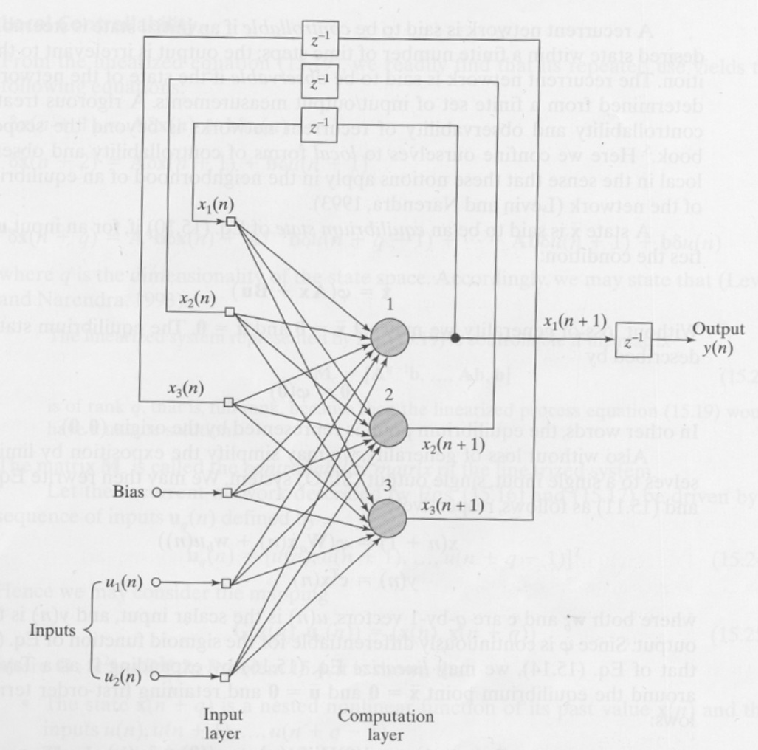
\includegraphics[width=11cm]{l12k9}

  \begin{solution}

    NARX is a nonlinear autoregressive exogenous model:
    \begin{align*}
      y_n = F(y_{n-1}, \ldots, y_{n-q}, \mathbf{x}_n, \mathbf{x}_{n-1},
      \ldots, \mathbf{x}_{n-p} ).
    \end{align*}
    In our case $F$ is modelled as a neural network, which is shown
    below.
    
    \begin{center}
      \usetikzlibrary{shapes}
      \usetikzlibrary{chains}
      \usetikzlibrary{arrows}
      \begin{tikzpicture}[start chain=hidden going below,
        start chain=input going below]

        \tikzset{>={triangle 45}}

        \tikzstyle{dot}=[draw,circle,fill,scale=0.4];
        \tikzstyle{box}=[draw,rectangle,scale=1.0];
        \tikzstyle{delay}=[draw,rectangle,minimum size=20pt];
        \tikzstyle{marker}=[minimum size=0pt, inner sep=0pt];
        \tikzstyle{neuron}=[draw,circle,fill=gray!25, minimum size=20pt];

        %%%%%%%%%%%%%
        % INPUT LAYER
        %%%%%%%%%%%%%

        % Time delays for input signal
        \node[dot] (xn) {};
        \node[marker, left=of xn, label=left:$x(n)$] (input) {};
        \node[delay, below=of xn] (z xn) {$z^{-1}$};
        \node[dot, below=of z xn, label=left:$x(n-1)$] (xn-1) {};
        \node[below=of xn-1] (xn dots) {$\vdots$};
        \node[dot,below=of xn dots, label=left:$x(n-p+1)$] (xn-p+1) {};
        \node[delay, below=of xn-p+1] (z xn-p+1) {$z^{-1}$};
        \node[marker,below=of z xn-p+1, label=left:$x(n-p)$] (xn-p) {};

        % Bias
        \node[marker, below=of xn-p] (bias) {};
        \node[marker,left=of bias, label=left:bias] (b) {};

        % Time delays for output signal
        \node[dot, below=of bias, label=left:$y(n-q)$] (yn-q) {};
        \node[delay, below=of yn-q] (z yn-q+1) {$z^{-1}$};
        \node[dot, below=of z yn-q+1, label=left:$y(n-q+1)$] (yn-q+1) {};
        \node[below=of yn-q+1] (yn dots) {$\vdots$};
        \node[dot,below=of yn dots, label=left:$y(n-1)$] (yn-1) {};
        \node[delay, below=of yn-1] (z yn) {$z^{-1}$};
        \node[marker,below=of z yn, label=left:$y(n)$] (yn recurrent) {};

        % Input nodes to the network
        \node[box, right=of xn] (u1) {};
        \node[box, right=of xn-1] (u2) {};
        \node[box, right=of xn-p+1] (u3) {};
        \node[box, right=of xn-p] (u4) {};

        % Bias node to the network
        \node[box, right=of bias] (u5) {};

        % Recurrent output nodes to the network
        \node[box, right=of yn-q] (u6) {};
        \node[box, right=of yn-q+1] (u7) {};
        \node[box, right=of yn-1] (u8) {};

        % Arrows in the input layer
        \draw[-] (input) -- (xn);
        \draw[->] (xn) -- (u1);
        \draw[->] (xn) -- (z xn);
        \draw[-] (z xn) -- (xn-1);
        \draw[->] (xn-1) -- (u2);
        \draw[->] (xn-1) -- (xn dots);
        \draw[-] (xn-p+1) -- (xn dots);
        \draw[->] (xn-p+1) -- (u3);
        \draw[->] (xn-p+1) -- (z xn-p+1);
        \draw[->] (z xn-p+1) -- (xn-p) -- (u4);

        % Arrow for bias
        \draw[->] (b) -- (u5);

        % Arrow for recurrent outputs
        \draw[->] (yn-q) -- (u6);
        \draw[-] (z yn-q+1) -- (yn-q);
        \draw[->] (yn-q+1) -- (z yn-q+1);
        \draw[->] (yn-q+1) -- (u7);
        \draw[-] (yn dots) -- (yn-q+1);
        \draw[->] (yn-1) -- (yn dots);
        \draw[->] (yn-1) -- (u8);
        \draw[-] (z yn) -- (yn-1);
        %\draw[-] (z yn) -- (yn recurrent);

        %%%%%%%%%%%%%%
        % HIDDEN LAYER
        %%%%%%%%%%%%%%

        % Neurons
        \node[neuron, right=3 of u3] (neuron1) {};
        \node[neuron, below=of neuron1] (neuron2) {};
        \node[neuron, below=of neuron2] (neuron3) {};
        \node[marker, below=of neuron3] (neuron dots) {$\vdots$};
        \node[neuron, below=of neuron dots] (neuron4) {};

        % Connections from the input layer to the hidden layer
        \foreach \i in {1,...,8} {
          \foreach \j in {1,...,4} {
            \draw[->] (u\i) -- (neuron\j);
          }
        }

        %%%%%%%%%%%%%%
        % OUTPUT LAYER
        %%%%%%%%%%%%%%

        \node[neuron, right=2 of neuron3] (neuron y) {};
        \node[dot, right=of neuron y] (dot yn) {};
        \node[right=of dot yn, label=right:$y(n)$] (yn) {};
        \draw[-] (neuron y) -- (dot yn);
        \draw[->] (dot yn) -- (yn);

        % Connections from the hidden layer to the output neuron
        \foreach \j in {1,...,4} {
          \draw[->] (neuron\j) to (neuron y);
        }
        \draw[->] (dot yn) |- (yn recurrent) -- (z yn);

        % % 
        % \foreach \i in {1,...,6} {
        %   \node[rectangle,draw] (in\i) at (0,2*7-2*\i) {};
        % }
        % \foreach \i in {1,...,3} {
        %   \node[circle,draw,fill=gray,minimum size=20pt] (hid\i) at (3,2*5.5-2*\i) {};
        % }
        % % 
        % % % Hidden layer
        % % \node[circle,fill=gray!25,draw,minimum
        % % size=20pt,on chain=hidden,label=1] (h1) {};
        % % \node[circle,fill=gray!25,draw,minimum
        % % size=20pt,on chain=hidden,label=2] (h2) {};
        % % \node[circle,fill=gray!25,draw,minimum
        % % size=20pt,on chain=hidden,label=3] (h3) {};
        % % 

        % % Output layer
        % \node[right=100pt of hid1]
        % (out) {$y(n)$};

        % % Arrows input->hidden
        % \foreach \i in {1,...,6} {
        %   \foreach \j in {1,...,3} {
        %     \draw[->] (in\i) -- (hid\j);
        %   }
        % }

        % % Arrow hidden->output
        % \draw[->] (hid1) -- (out);

        % % Recurrent arrows
        % \foreach \i in {1,2,3} {
        %   % Unit time-delays
        %   \path (hid\i) ++(-1.5,3*\i+2) node[draw,rectangle,minimum
        %   size=20pt] (z\i) {$z^{-1}$};
        %   % Arrows
        %   \draw[->] (hid\i) -- ++(1.5+\i*0.5,0) node[at start,label=above
        %   right:$x_\i(n)$] {} node (crossing\i) {} -- ++(0,3*\i+2) --
        %   (z\i) -- ++(-\i*0.5-3,0) node (current) {} -- (current |- in\i)
        %   -- (in\i) node[at end, label=above left:$x_\i(n-1)$] {};
        % }

        % \node[circle,draw,fill,scale=0.4] at (crossing1) {};

        % \draw[<-] (in4) -- ++(-1,0) node[label=left:$1$] {};
        % \draw[<-] (in5) -- ++(-1,0) node[label=left:$u_1(n)$] {};
        % \draw[<-] (in6) -- ++(-1,0) node[label=left:$u_2(n)$] {};
        
      \end{tikzpicture}
    \end{center}
    

  \end{solution}

\end{enumerate}
\end{document}             % End of document.

%%% Local Variables: 
%%% mode: latex
%%% TeX-master: "ex11_solutions"
%%% End: 
